% 若编译失败，且生成 .synctex(busy) 辅助文件，可能有两个原因：
% 1. 需要插入的图片不存在：Ctrl + F 搜索 'figure' 将这些代码注释/删除掉即可
% 2. 路径/文件名含中文或空格：更改路径/文件名即可

% --------------------- 文章宏包及相关设置 --------------------- %
% >> ------------------ 文章宏包及相关设置 ------------------ << %
% 设定文章类型与编码格式
\documentclass[UTF8]{article}		
\input{../.config/config_for_MCPExperiment.tex}



%%%%%%%%%%%%%%%%%%%%%%%%%%%%%%%%%%%%%%%%%%%%%%%%%%%%%%%%%%%%%%%%
% 仅需修改页眉、实验名称、实验日期
%%%%%%%%%%%%%%%%%%%%%%%%%%%%%%%%%%%%%%%%%%%%%%%%%%%%%%%%%%%%%%%%


%%%%%%%%%%%%%%%%%% 1. 修改页眉内容 %%%%%%%%%%%%%%%%%%
\rhead{MCP-06 并行端口 \& LCD 显示 (2025.12.17, 徐睿琳)}

% 开始编辑文章
\begin{document}
\begin{center}\large
    \vspace*{-0.8cm}
    \noindent{\huge\bfseries《\ \ 微\ \ 机\ \ 原\ \ 理\ \ 实\ \ 验\ \ \ 》\ \ 实\ \ 验\ \ 报\ \ 告 }
    \\\vspace{0.1cm}
    \noindent{
    {\bfseries 
%
%%%%%%%%%%%%%%%%%% 2. 修改实验名称 %%%%%%%%%%%%%%%%%%
    实验名称：\uline{\hspace{2.2cm} 并行端口 \& LCD 显示 \hspace{2.2cm}}
%
    }\hspace{0.4cm}
    指导教师：\uline{\hspace{0.8cm}肖山林     \hspace{0.8cm}}
    }
    \\\vspace{0.1cm}
    \noindent
    {
    姓名：\uline{\,\,\,徐睿琳\,\,\,}\hspace{0.2cm}
    学号：\uline{\,\,\,{ 23342107}\,\,\,}\hspace{0.2cm}
    专业/班级：\uline{\,\,\,{微电子/三班}\,\,\,}\hspace{0.2cm}
    分组序号：\uline{\,\,\,{A412-A05}\,\,\,}
    }
    \\\vspace{0.1cm}
    \noindent{
%
%%%%%%%%%%%%%%%%%% 3. 修改实验日期 %%%%%%%%%%%%%%%%%%
    实验日期：\uline{\,\,{2025.12.17}\,\,}\hspace{0.2cm}
%
    实验地点：\uline{\,\,\,教学楼{ A412}\,\,\,}\hspace{0.2cm}
    是否调课/补课：\uline{\hspace{0.26cm}否 \hspace{0.26cm}}\hspace{0.2cm}
    成绩：\uline{\hspace{2cm}}
    }
\end{center}
\vspace{-0.4cm}
\noindent\rule{\textwidth}{0.075em}   % 分割线
\vspace{-1.0cm}

% 生成目录
\setcounter{tocdepth}{3}  % 目录深度为 2（不显示 subsubsection）
\noindent\tableofcontents\thispagestyle{fancy}   % 显示页码、页眉等

% ------------------------ 文章信息区 ------------------------ %
% ------------------------ 文章信息区 ------------------------ %



%%%%%%%%%%%%%%%%%%%%%%%%%%%%%%%%%%%%%%%%%%%%%%%%%%%%%%%%%%%%%%%%%%%%%%%%%%%%%%%%%
%%%%%%%%%%%%%%%%%%%%%%%%%%%%%%%%% 下面是正文内容 %%%%%%%%%%%%%%%%%%%%%%%%%%%%%%%%%
%%%%%%%%%%%%%%%%%%%%%%%%%%%%%%%%%%%%%%%%%%%%%%%%%%%%%%%%%%%%%%%%%%%%%%%%%%%%%%%%%

\section{实验内容与设计}

\subsection{8255A 控制 LED 显示}

\begin{figure}[H]
  \centering
  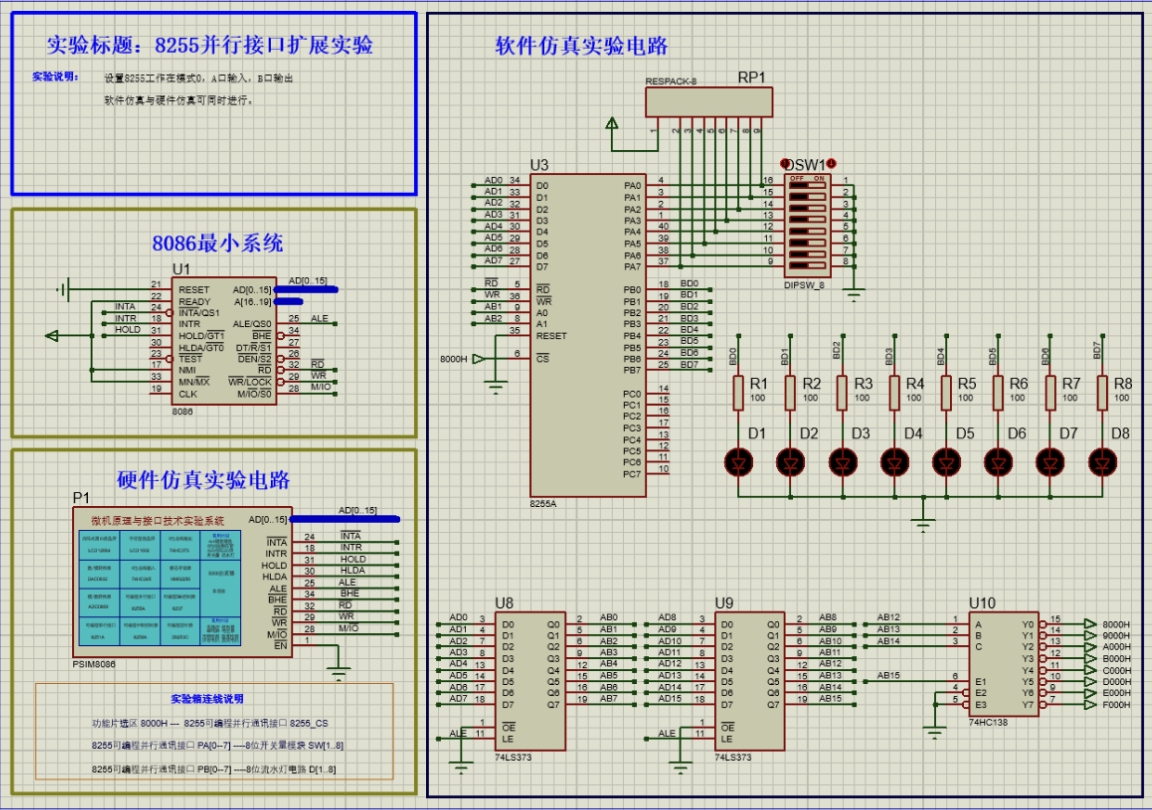
\includegraphics[width=0.8\textwidth]{images/image-2025-12-22-15-57-20.png}
  \caption{电路原理图}
  \label{fig:image-2025-12-22-15-57-20.png}
\end{figure}

\begin{bluebox}
我们通过配置 8255A 的工作方式，将其 PB 端口（IOB）和 PC 端口（IOC）分别用于控制 8 个 LED 灯中的不同部分。具体做法如下：

\begin{itemize}
    \item 8255A 被设置为 A 口输入，B 口和 C 口输出（控制字 90H）。
    \item 程序每次从 A 口读取 8 位数据，将高 4 位（AL7~AL4）通过与操作（AND 0F0H）送到 PB 端口，控制前 4 个 LED（LED1~LED4）。
    \item 低 4 位（AL3~AL0）通过与操作（AND 0FH）送到 PC 端口，控制后 4 个 LED（LED5~LED8）。
\end{itemize}

这样，PB 端口的 4 位输出直接对应前 4 个 LED 的亮灭，PC 端口的 4 位输出对应后 4 个 LED，实现了分端口独立控制。
\end{bluebox}

\begin{lstlisting}[language={[x86masm]Assembler}]
    CODE    SEGMENT                 
        ASSUME CS:CODE              

    ; 8255A 端口地址定义
    IOCON   EQU 08006H              ; 控制口地址
    IOA     EQU 08000H              ; A 口地址
    IOB     EQU 08002H              ; B 口地址
    IOC     EQU 08004H              ; C 口地址

    START:                          
        MOV AL,90H                  ; A 口输入，B/C 口输出
        MOV DX,IOCON                
        OUT DX,AL                   

    START1:                         
        MOV AL,0                    
        MOV DX,IOA                  
        IN AL,DX                    

        MOV BL,AL                   
        MOV DX,IOB                  
        AND AL,0F0H                 ; 保留高 4 位（AL7~AL4），低 4 位清零
        OUT DX,AL                   

        AND BL,0FH                  ; 保留低 4 位（BL3~BL0），高 4 位清零
        MOV AL,BL                   
        MOV DX,IOC                  
        OUT DX,AL                   

        JMP START1                  

    CODE    ENDS                    
        END START                   
\end{lstlisting}

\subsection{LCD 显示字符}

\begin{figure}[htbp]
  \centering
  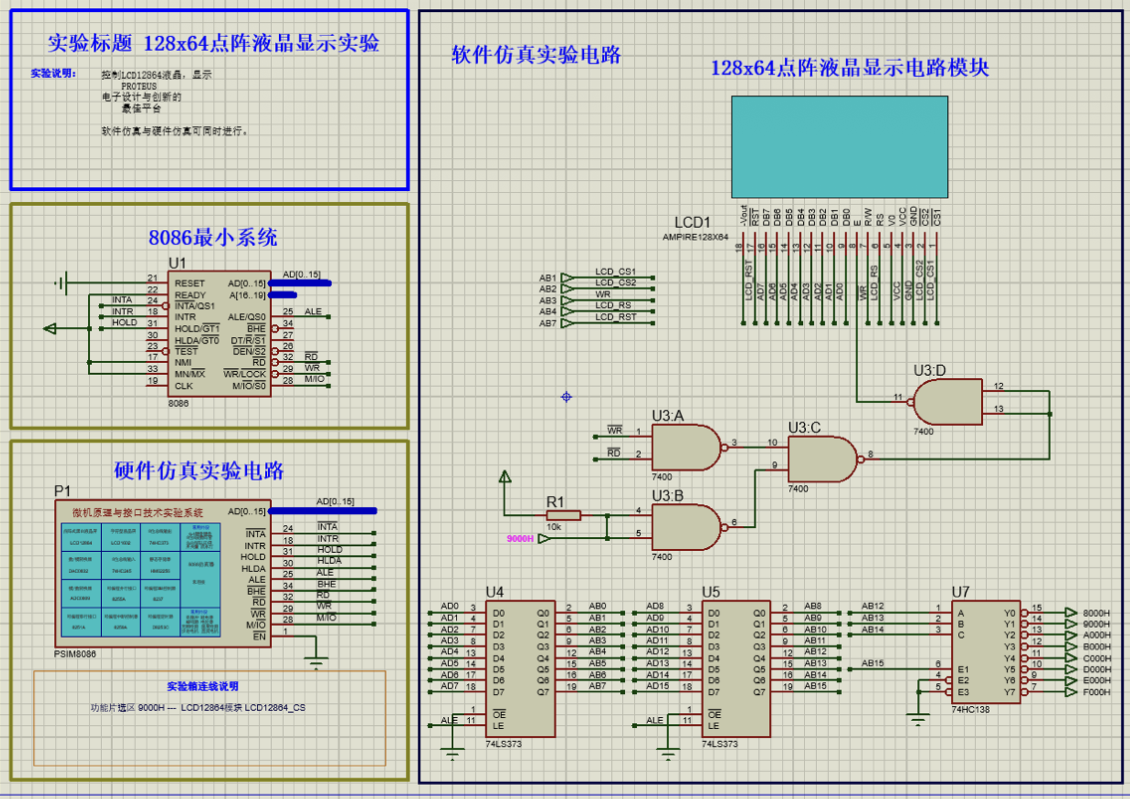
\includegraphics[width=0.8\textwidth]{images/image-2025-12-22-16-06-11.png}
  \caption{LCD 显示字符电路原理图}
  \label{fig:image-2025-12-22-16-06-11.png}
\end{figure}

\begin{bluebox}
我们先对液晶模块进行复位与初始化，设置起始行、页和列，并打开显示模式。字符点阵保存在 DATA 段：英文/数字用 8×16 点阵（ZF\_x 系列），中文用 16×16 点阵（TABLE\_HZ / TABLE\_HZ2）。

显示时通过封装的写字符例程来完成：调用写字符串例程依次取出每个字符的点阵地址，并调用通用写字符子程序。写字符子程序根据传入参数（字符宽度 AX=8/16、X 地址 BL、Y 地址 BH、点阵首地址 DI）先发送设置坐标的指令，再根据当前列所在的屏（高位）选择相应的数据端口，将点阵字节逐列输出到 LCD。输出完成后更新列/页坐标，继续下一字符。

因此，只需在 DATA 中准备好学号与姓名对应的点阵并调用相应的字符串写入例程，LCD 即可在指定位置连续显示学号与姓名。
\end{bluebox}

\begin{lstlisting}[language={[x86masm]Assembler}]
CODE    SEGMENT 'CODE'
       ASSUME DS:DATA,CS:CODE,SS:STACK
       
       LCD_CMD_WR​EQU ​9086H
       LCD_DATA_WR1​EQU​9092H    ;写第一屏数据
       LCD_DATA_WR2​EQU​9094H    ;写第二屏数据
       LCD_DATA_WR0​EQU​9096H    ;写双屏数据
       LCD_DATA_RD​EQU​909EH
       LCD_RST         EQU     9000H    ;复位
       LCD_RST_OK      EQU     9080H    ;复位
 
 
       LCD_ROW         EQU     0C0H     ;设置起始行
       LCD_PAGE        EQU     0B8H    ;设置起始页
       LCD_COLUMN      EQU     40H     ;设置起始列
       LCD_PAGE_MAX    EQU     08H     ;页数最大值
       LCD_COLUMN_MAX  EQU     40H     ;列数最大值
 
START:
       MOV AX, DATA
       MOV DS, AX
 
       MOV AX, STACK
       MOV SS, AX
 
       MOV AX, TOP
       MOV SP, AX
 
       CALL LCD_INIT
 
       CALL LCD_CLEAR
 
MAINLOOP:
       CALL WRSTR_PROTEUS
 
       CALL WRHZ
​
​CALL WRSTR_PROTEUS2
​
​CALL WRHZ2
 
       JMP START
       
LCD_INIT:        
       MOV DX, LCD_RST
       OUT DX, AL
 
       MOV AL, 00H
       MOV DX, LCD_RST_OK
       OUT DX, AL
 
       IN  AL, DX    
 
       MOV AL, LCD_ROW
       CALL WRCMD
 
       MOV AL, LCD_COLUMN
       CALL WRCMD
 
       MOV AL, LCD_PAGE
       CALL WRCMD
       
       MOV AL, 3FH
       CALL WRCMD
       RET
       
LCD_CLEAR:
       MOV BL, 00H
LC_LOOP:MOV AL, BL
       ADD AL, LCD_PAGE
       CALL WRCMD
       MOV AL, LCD_COLUMN
       CALL WRCMD
       MOV CX, LCD_COLUMN_MAX
       MOV AL, 00H
       MOV DX, LCD_DATA_WR0
LC_WDATA:
       OUT DX, AL
       LOOP LC_WDATA
       INC BL
       CMP BL, LCD_PAGE_MAX
       JL LC_LOOP
       RET
 
WRCMD:  PUSH DX
       MOV DX, LCD_CMD_WR
       OUT DX, AL
       POP DX
       RET
       
WRSTR_PROTEUS:
       MOV AX, 8
       MOV CX, 8
       MOV BX, 0028H
       LEA DI, ZF_1
 
WRSTR_LOOP:
       CALL WRCHAR
       ADD BX, AX
       ADD DI, 16
       LOOP WRSTR_LOOP
       RET
WRSTR_PROTEUS2:
       MOV AX, 8
       MOV CX, 8
       MOV BX, 0428H
       LEA DI, ZF_9
WRSTR_LOOP2:
       CALL WRCHAR
       ADD BX, AX
       ADD DI, 16
       LOOP WRSTR_LOOP
       RET
       
WRHZ:
       MOV AX, 16
       MOV CX, 3
       MOV BX, 0230H
       LEA DI, TABLE_HZ
 
WRHZ_LOOP:
       CALL WRCHAR
       ADD BX, AX
       ADD DI, 32
       LOOP WRHZ_LOOP
​RET
 
WRHZ2:
       MOV AX, 16
       MOV CX, 3
       MOV BX, 0630H
       LEA DI, TABLE_HZ2
 
WRHZ_LOOP2:
       CALL WRCHAR
       ADD BX, AX
       ADD DI, 32
       LOOP WRHZ_LOOP2    
​RET
​
 
;入口参数：
;AX-->字符宽度，ASCII为8，汉字为16
;BL-->X地址，0-127
;BH-->Y地址，0-7
;DI-->字符首地址
WRCHAR: PUSH AX
       PUSH BX
       PUSH CX
       PUSH DX
       PUSH DI
       MOV CX,AX
       MOV AH, 02H
       ADD BL, LCD_COLUMN
       ADD BH, LCD_PAGE
WRCHAR_P:
       MOV AL,BH
       CALL WRCMD
       TEST BL, 80H
       JNZ  WRCHAR_P0
       MOV AL, BL
       CALL WRCMD
       MOV DX, LCD_DATA_WR1
       JMP WRCHAR_P1
WRCHAR_P0:
       MOV AL, BL
       SUB AL, 40H
       CALL WRCMD
       MOV DX, LCD_DATA_WR2
WRCHAR_P1:
       PUSH CX
WRBIT1: MOV AL, [DI]
       OUT DX, AL
       INC DI
       LOOP WRBIT1
       POP CX
       INC BH
       MOV AL,00H
       XCHG AL,AH
       DEC AX
       XCHG AL,AH
       JNZ WRCHAR_P
       POP DI
       POP DX
       POP CX
       POP BX
       POP AX
WRRET:  RET
 
CODE    ENDS
 
STACK   SEGMENT 'STACK'
STA     DB  100 DUP(?)
TOP     EQU LENGTH STA
STACK   ENDS
 
       END START
\end{lstlisting}

\subsection{8255A 控制 7 位数码管显示}

\begin{figure}[H]
  \centering
  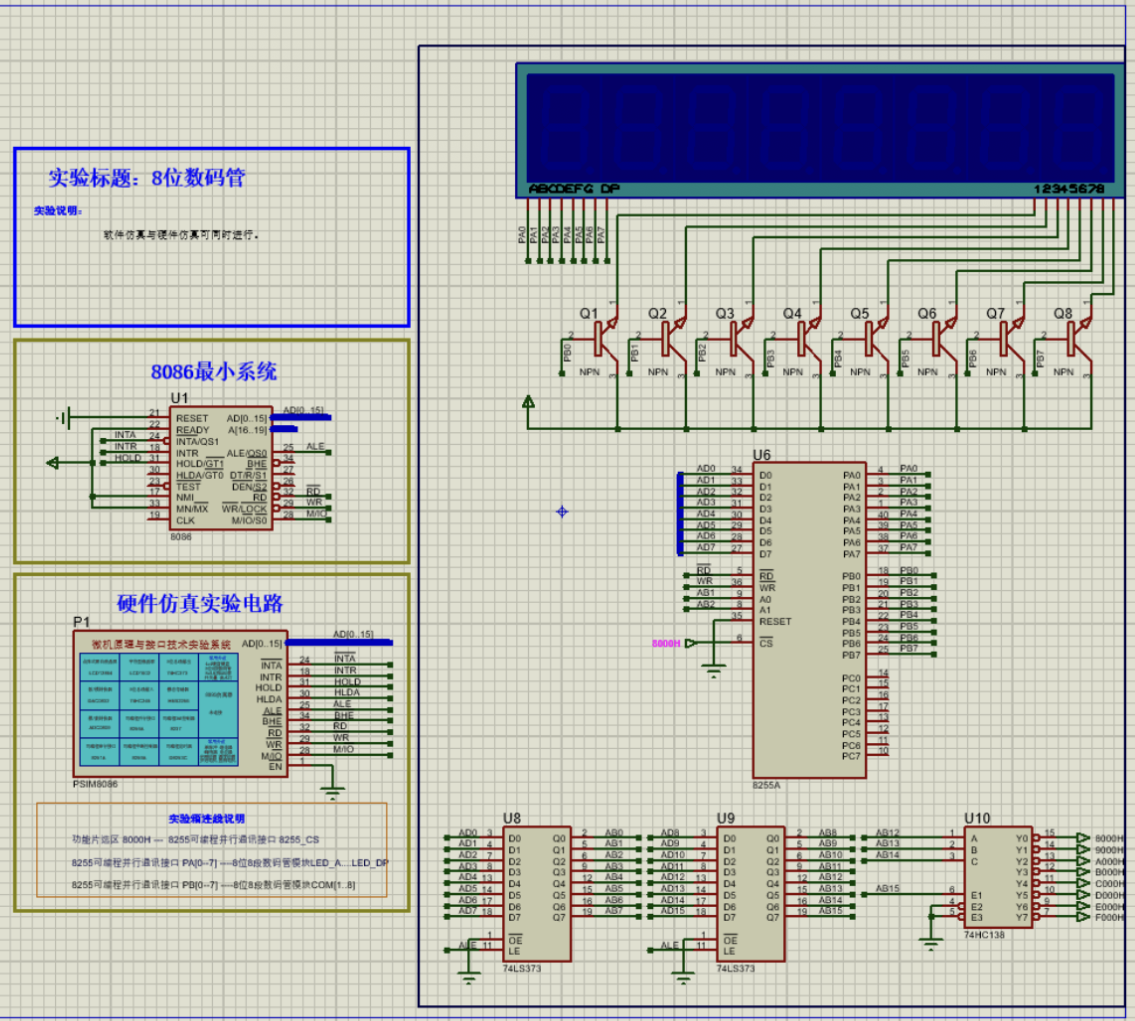
\includegraphics[width=0.8\textwidth]{images/image-2025-12-22-16-15-48.png}
  \caption{7 位数码管显示电路原理图}
  \label{fig:image-2025-12-22-16-15-48.png}
\end{figure}

\begin{bluebox}
我们通过将8255A配置为方式0、A/B/C口均为输出（控制字80H），用端口A作段选（段码），端口B作位选（位选），实现对共阳/共阴（本实验为共阳）7段数码管的多路复用扫描显示。程序在DATA段准备好每一位对应的段码表，循环8次依次显示8个数码管：先向端口B输出0（消隐）关闭所有数码管，向端口A输出当前位的段码，再向端口B输出对应的位选信号选通当前数码管，短暂保持后右移位选掩码以选通下一位并读取下一个段码。通过高速循环刷新（轮询每位并不断重复），利用人眼的暂留效应得到完整的实验日期显示。\colorbox{yellow}{\parbox{\linewidth}{为避免残影，单次切换时先消隐再写段码再点亮位选；位选由BH寄存器保存并每次右移以实现逐位扫描。}}
\end{bluebox}

\begin{lstlisting}[language={[x86masm]Assembler}]
CODE    SEGMENT 'CODE'
       ASSUME CS:CODE,SS:STACK,DS:DATA
       
IOCON   EQU 8006H      ; 8255控制寄存器端口
IOA     EQU 8000H      ; 8255端口A
IOB     EQU 8002H      ; 8255端口B
IOC     EQU 8004H      ; 8255端口C
 
START:
       MOV AX, DATA   ; 初始化数据段
       MOV DS, AX
 
       MOV AX, STACK  ; 初始化堆栈段
       MOV SS, AX
 
       MOV AX, TOP    ; 设置堆栈指针（这里有问题）
       MOV SP, AX     ; 应该用 MOV SP, offset TOP
       
       
TEST_BU:
       MOV AL,80H     ; 8255控制字：方式0，A/B/C口都输出
       MOV DX,IOCON
       OUT DX,AL      ; 写入8255控制寄存器
       NOP            ; 短暂延时
       
RESET:  
       LEA DI,TABLE   ; DI指向显示数据表
       MOV CX,08H     ; 循环8次（8个数码管）
       MOV BH,80H     ; BH=10000000B（从最高位数码管开始）
       
DISPLA2:
       MOV DX,IOB     ; 准备写端口B（位选）
       MOV AL,00H     ; 先关闭所有数码管（消隐）
       OUT DX,AL      ; 输出到位选端口
       
       MOV DX,IOA     ; 准备写端口A（段选）
       MOV AL,[DI]    ; 读取显示数据
       OUT DX,AL      ; 输出到段选端口
       
       MOV DX,IOB     ; 再次写端口B
       MOV AL,BH      ; 取位选信号
       OUT DX,AL      ; 选通当前数码管
       
       INC DI         ; 指向下一个显示数据
       MOV AL,BH      ; 当前位选信号
       SHR AL,1       ; 右移一位，选通下一个数码管
       MOV BH,AL      ; 保存到位选寄存器
       
       LOOP DISPLA2   ; 循环显示8个数码管
       
       JMP RESET      ; 无限循环
 
CODE    ENDS
     
STACK   SEGMENT 'STACK'
STA     DB  100 DUP(?) ; 100字节堆栈空间
TOP     EQU LENGTH STA ; TOP=100（堆栈长度）
STACK   ENDS      
     
DATA    SEGMENT 'DATA'
TABLE   DB 0F8H,0F9H,0A4H,0F9H,92H,0A4H,0C0H,0A4H
 
       ; 数码管显示数据（共阳极）：
DATA    ENDS
       END START      ; 程序结束，从START开始执行
\end{lstlisting}

\section{实验结果}

\subsection{8255A 控制 LED 显示}

\begin{figure}[H]
    \centering
    \begin{subfigure}[b]{0.32\textwidth}
        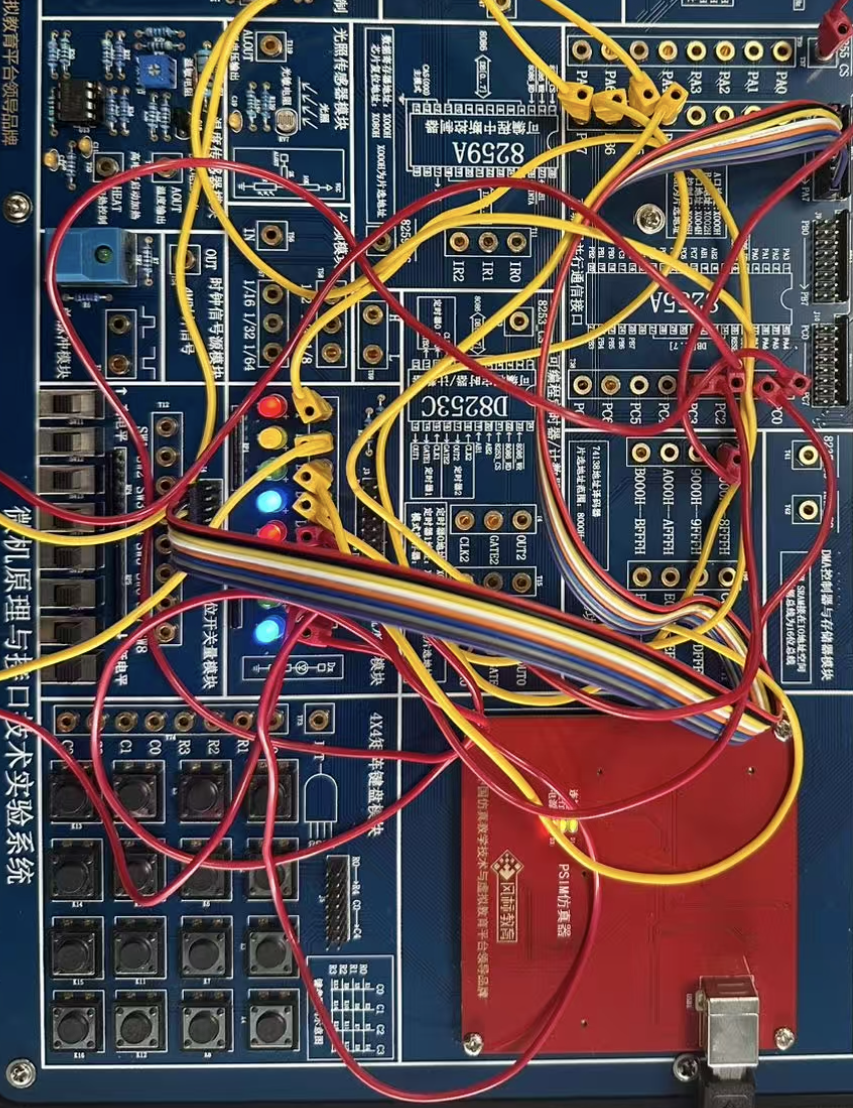
\includegraphics[width=\textwidth]{images/image-2025-12-22-15-59-05.png}
        \caption{LED 显示效果 1}
        \label{fig:image-2025-12-22-15-59-05.png}
    \end{subfigure}
    \hfill
    \begin{subfigure}[b]{0.32\textwidth}
        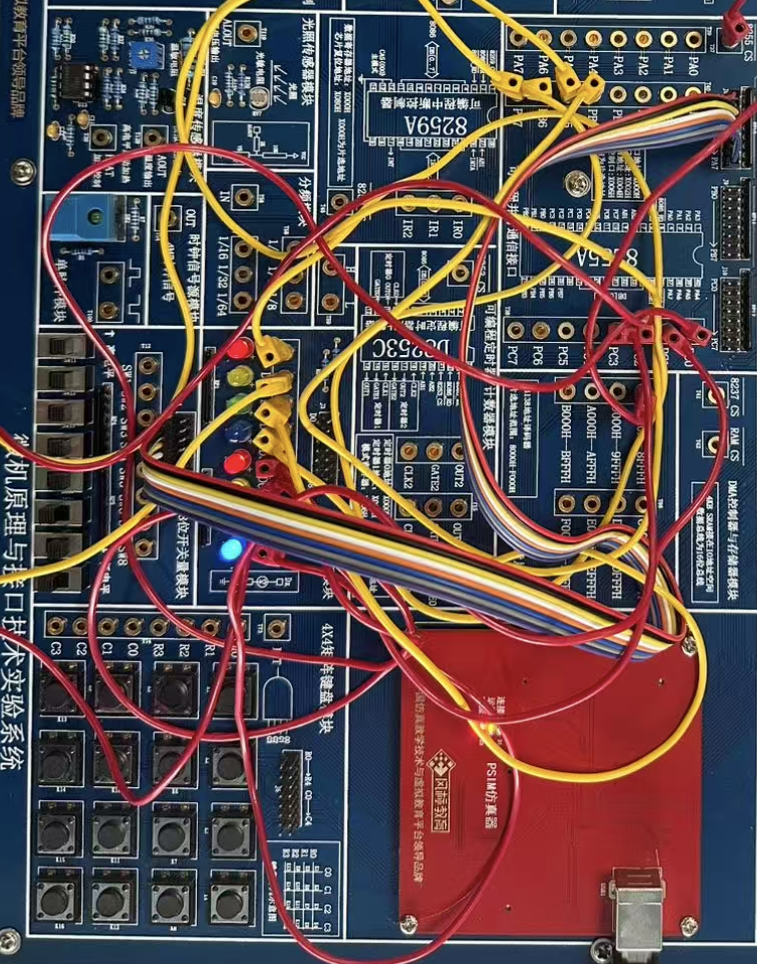
\includegraphics[width=\textwidth]{images/image-2025-12-22-15-59-24.png}
        \caption{LED 显示效果 2}
        \label{fig:image-2025-12-22-15-59-24.png}
    \end{subfigure}
    \hfill
    \begin{subfigure}[b]{0.32\textwidth}
        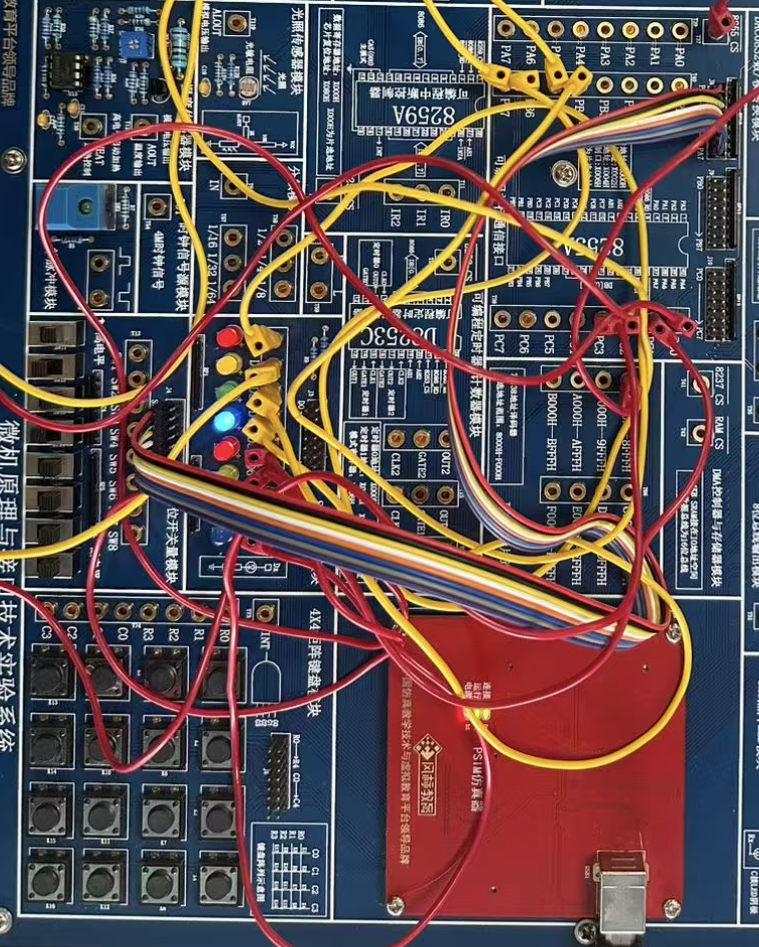
\includegraphics[width=\textwidth]{images/image-2025-12-22-15-59-37.png}
        \caption{LED 显示效果 3}
        \label{fig:image-2025-12-22-15-59-37.png}
    \end{subfigure}
    \caption{LED 显示效果}
\end{figure}

\subsection{LCD 显示字符}

\begin{figure}[H]
  \centering
  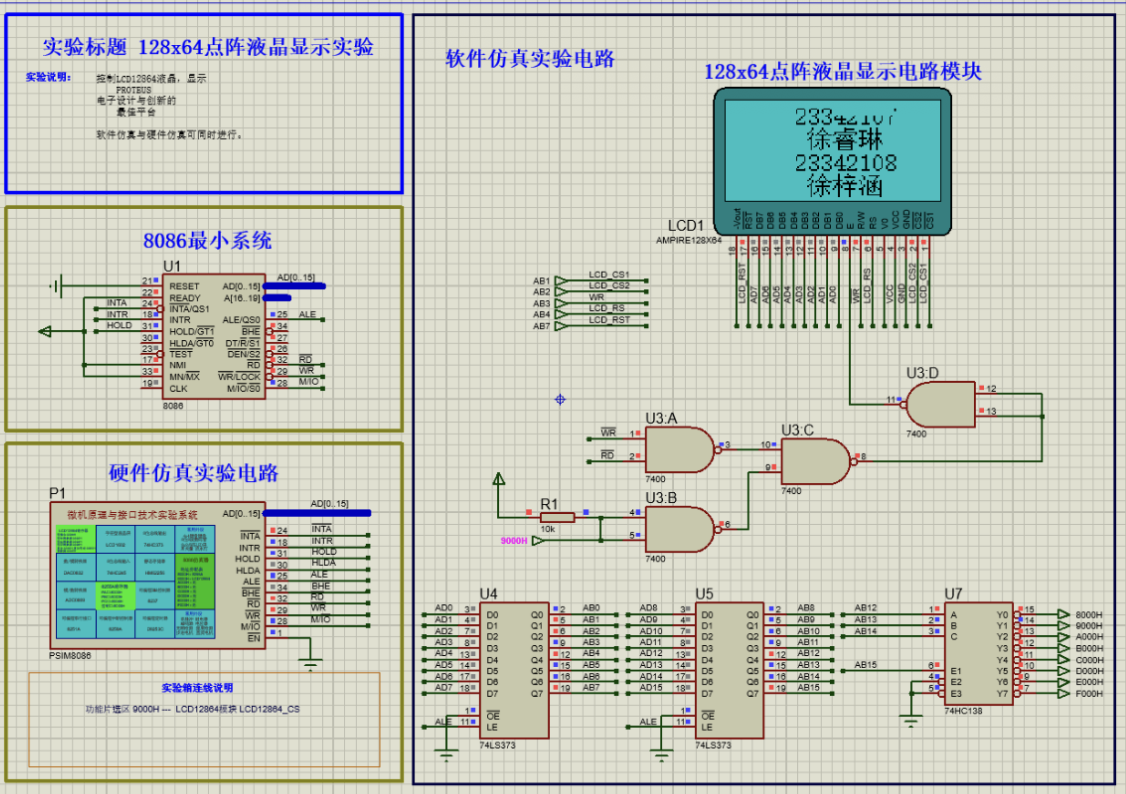
\includegraphics[width=0.8\textwidth]{images/image-2025-12-22-16-14-37.png}
  \caption{LCD 显示仿真软件截图}
  \label{fig:image-2025-12-22-16-14-37.png}
\end{figure}

\begin{figure}[H]
    \centering
    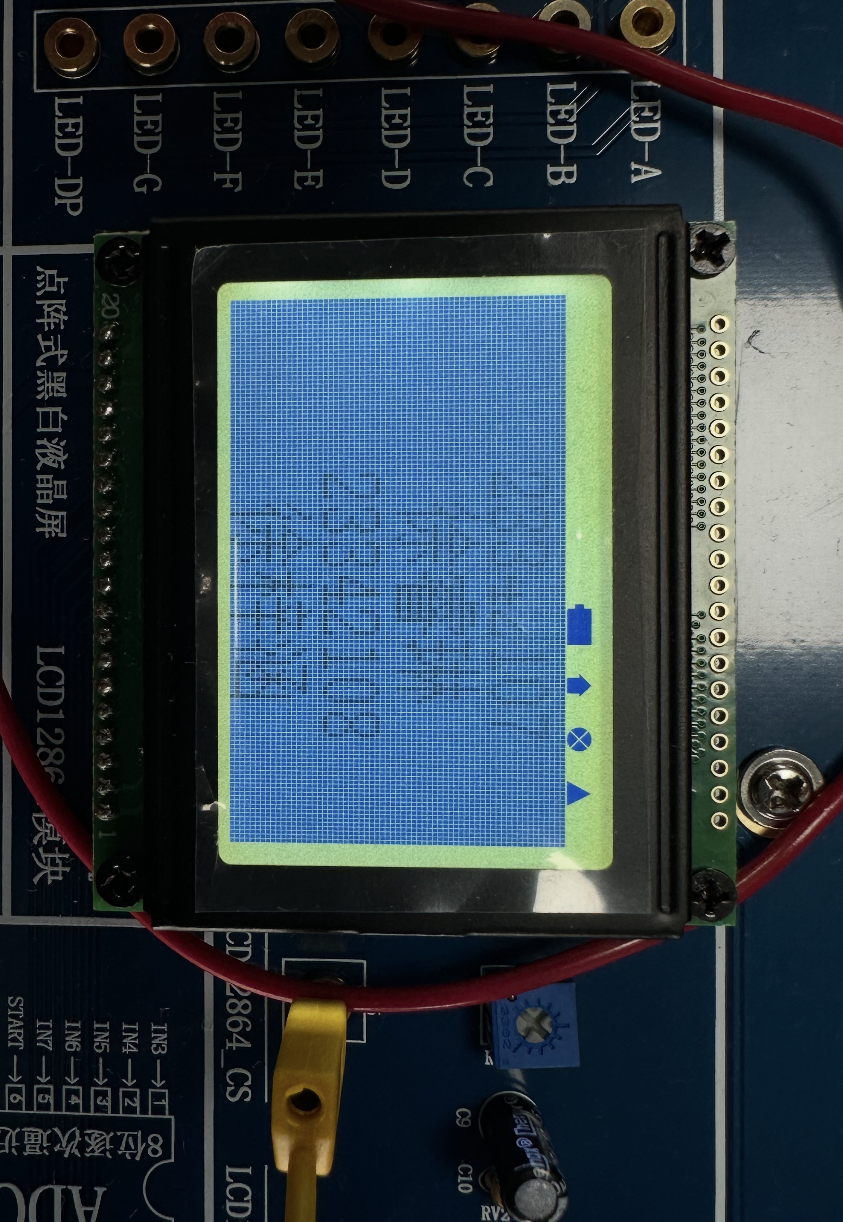
\includegraphics[width=0.5\textwidth, angle=90]{images/image-2025-12-22-16-01-23.png}
    \caption{学号-姓名 LCD 显示效果}
    \label{fig:image-2025-12-22-16-01-23.png}
\end{figure}

\subsection{8255A 控制 7 位数码管显示}



\begin{figure}[H]
  \centering
  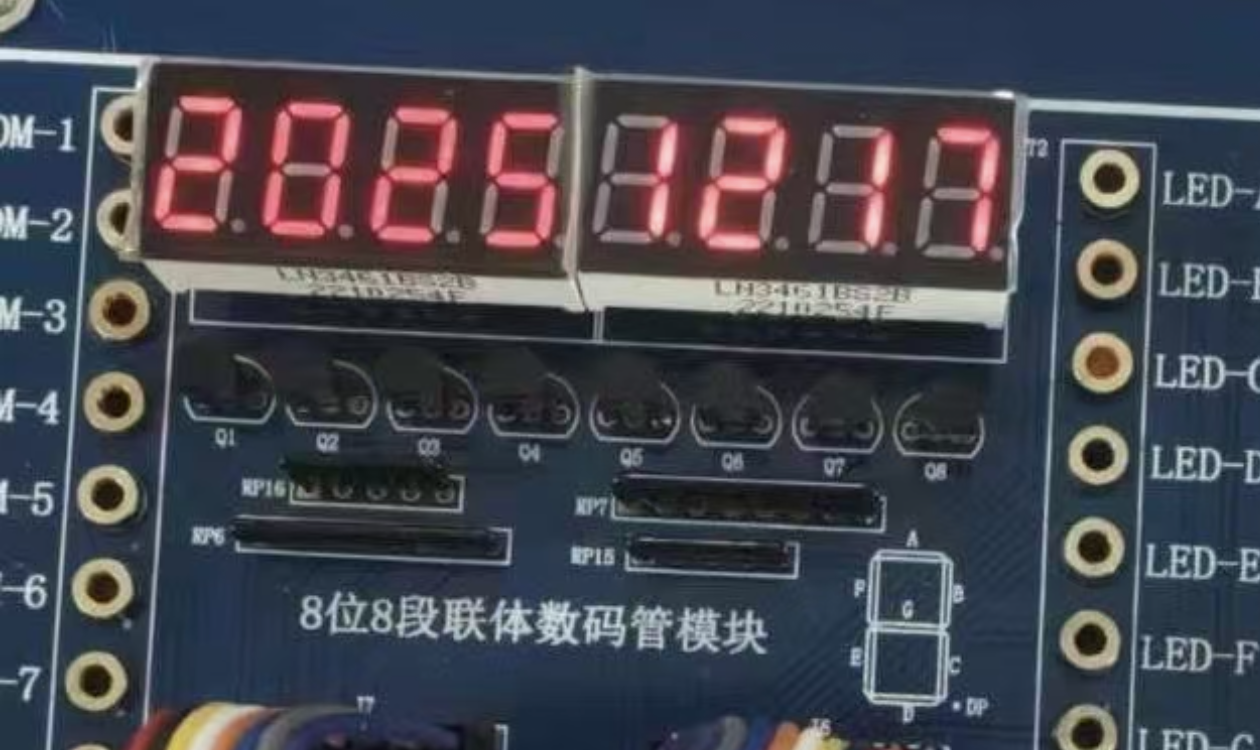
\includegraphics[width=0.8\textwidth]{images/image-2025-12-22-16-03-24.png}
  \caption{实验日期显示效果}
  \label{fig:image-2025-12-22-16-03-24.png}
\end{figure}

\section{思考与总结}

\subsection{实验总结}

通过本次实验，我深入理解了 8255A 并行接口芯片的工作原理及其在 Mode 0 下的配置方法，并掌握了微机系统与外部显示设备交互的基本时序控制。

\begin{itemize}
    \item \textbf{8255A 端口控制}：在 LED 控制实验中，掌握了如何通过控制字将 8255A 的不同端口分别配置为输入和输出。理解了 CPU 通过数据总线读取开关状态并处理后输出到 LED 的完整流程。
    \item \textbf{LCD 液晶显示}：熟悉了点阵式 LCD 的初始化序列、页/列地址设置以及汉字点阵的提取与写入方法。特别是理解了“字模”是如何映射到屏幕像素点的，以及如何通过循环调用子程序实现字符串的连续显示。
    \item \textbf{数码管动态扫描}：在数码管实验中，深刻体会了“动态扫描”的设计思想。通过快速轮流选通各个数码管并送入对应的段码，利用人眼的视觉暂留效应实现了多位数字的同时显示。同时，实验中也验证了在位选切换前进行“消隐”操作对于消除显示残影（鬼影）的重要性。
\end{itemize}

\subsection{鲁棒性提升方案：LCD 忙标志检测}

\subsubsection{问题分析}
在当前的 LCD 显示程序中，我们在写入指令（\texttt{WRCMD}）或数据时，主要依赖于指令执行间的自然延时或简单的循环等待。然而，LCD 控制器（如 T6963C 或兼容芯片）处理指令内部需要一定的时间周期。如果 CPU 主频较高或写入速度过快，超过了 LCD 的处理能力，前一条指令尚未执行完毕就写入下一条，极易导致显示乱码、丢字或花屏。

为了提高程序的\textbf{鲁棒性}（Robustness），使其能适应不同速度的 CPU 或不同响应特性的 LCD 模块，标准的做法是在每次写入操作前，通过软件轮询 LCD 的状态寄存器，检测其是否处于“忙”状态。

\subsubsection{改进代码实现}
可以通过读取 LCD 的状态端口（通常与指令写入端口地址相同，但操作为读）来判断。对于 T6963C 控制器，状态字的低两位（STA0 和 STA1）通常表示指令读写和数据读写的能力。

\textbf{改进思路}：编写一个 \texttt{CHECK\_BUSY} 子程序，在 \texttt{WRCMD} 和写数据前调用，确保 LCD 就绪后再进行输出。

\begin{lstlisting}[language={[x86masm]Assembler}]
; ---------------------------------------------------------
; 改进后的 LCD 写指令子程序 (增加忙检测)
; ---------------------------------------------------------
WRCMD_SAFE: 
       PUSH AX
       PUSH DX
       
       CALL CHECK_BUSY  ; 关键改进：先检测忙状态，等待就绪
       
       MOV DX, LCD_CMD_WR
       OUT DX, AL       ; 确认不忙后，再安全写入指令
       
       POP DX
       POP AX
       RET

; ---------------------------------------------------------
; 判忙子程序 (Check Busy Status)
; ---------------------------------------------------------
CHECK_BUSY:
       PUSH AX
       PUSH DX
       MOV DX, LCD_CMD_WR   ; 读状态通常使用指令口的读操作
       
WAIT_FOR_IDLE:
       IN AL, DX            ; 读取状态字
       AND AL, 03H          ; 屏蔽高位，只保留 STA0, STA1
                            ; STA0=1: 指令读写有效
                            ; STA1=1: 数据读写有效
       CMP AL, 03H          ; 检查是否两位都为 1
       JNE WAIT_FOR_IDLE    ; 如果不等于 03H (即忙)，则循环等待
       
       POP DX
       POP AX
       RET
\end{lstlisting}

\begin{bluebox}
通过加入上述 \texttt{CHECK\_BUSY} 机制，程序不再依赖不可靠的硬延时，而是根据硬件的实际反馈来决定执行节奏。这不仅解决了潜在的时序冲突问题，也使得代码在移植到更高主频的实验箱或实际工程中时，依然能稳定运行。
\end{bluebox}

% \subsection*{4.1 \ \ }
% \subsection*{4.2 \ \ }
% \subsection*{4.3 \ \ }
% \subsection*{4.4 \ \ }
% \subsection*{4.5 \ \ }
% \subsection*{4.6 \ \ }




















































\newpage
% 附录
\section*{附录 A\hspace*{20pt} 学号-姓名字符表}
\addcontentsline{toc}{section}{附录 A\hspace*{6pt} 学号-姓名字符表} 
\thispagestyle{fancy} 

\begin{lstlisting}[language={[x86masm]Assembler}]

DATA    SEGMENT 'DATA'
;--  文字:  2  --
;--  宋体12;  此字体下对应的点阵为：宽x高=8x16   --
ZF_1 DB  00H,70H,08H,08H,08H,08H,0F0H,00H,00H,30H,28H,24H,22H,21H,30H,00H
 
;--  文字:  3  --
;--  宋体12;  此字体下对应的点阵为：宽x高=8x16   --
ZF_2 DB  00H,30H,08H,08H,08H,88H,70H,00H,00H,18H,20H,21H,21H,22H,1CH,00H
 
;--  文字:  3  --
;--  宋体12;  此字体下对应的点阵为：宽x高=8x16   --
ZF_3 DB  00H,30H,08H,08H,08H,88H,70H,00H,00H,18H,20H,21H,21H,22H,1CH,00H
 
;--  文字:  4  --
;--  宋体12;  此字体下对应的点阵为：宽x高=8x16   --
ZF_4 DB  00H,00H,80H,40H,30H,0F8H,00H,00H,00H,06H,05H,24H,24H,3FH,24H,24H
 
;--  文字:  2  --
;--  宋体12;  此字体下对应的点阵为：宽x高=8x16   --
ZF_5 DB  00H,70H,08H,08H,08H,08H,0F0H,00H,00H,30H,28H,24H,22H,21H,30H,00H
 
;--  文字:  1  --
;--  宋体12;  此字体下对应的点阵为：宽x高=8x16   --
ZF_6 DB  00H,00H,10H,10H,0F8H,00H,00H,00H,00H,00H,20H,20H,3FH,20H,20H,00H
 
;--  文字:  0  --
;--  宋体12;  此字体下对应的点阵为：宽x高=8x16   --
ZF_7 DB  00H,0E0H,10H,08H,08H,10H,0E0H,00H,00H,0FH,10H,20H,20H,10H,0FH,00H
 
;--  文字:  7  --
;--  宋体12;  此字体下对应的点阵为：宽x高=8x16   --
ZF_8 DB  00H,18H,08H,08H,88H,68H,18H,00H,00H,00H,00H,3EH,01H,00H,00H,00H
 
 
;--  文字:  徐  --
;--  宋体12;  此字体下对应的点阵为：宽x高=16x16   --
TABLE_HZ DB  10H,88H,0C4H,33H,00H,20H,10H,28H,24H,0E3H,24H,28H,10H,20H,20H,00H
DB  01H,00H,0FFH,00H,20H,11H,0DH,41H,81H,7FH,01H,05H,09H,31H,00H,00H
 
;--  文字:  睿  --
;--  宋体12;  此字体下对应的点阵为：宽x高=16x16   --
DB  20H,18H,88H,0A8H,68H,28H,0A8H,6FH,0AAH,2AH,6AH,0AAH,0AH,28H,18H,00H
DB  04H,04H,02H,0FEH,0ABH,0ABH,0AAH,0AAH,0AAH,0ABH,0ABH,0FEH,02H,04H,04H,00H
 
;--  文字:  琳  --
;--  宋体12;  此字体下对应的点阵为：宽x高=16x16   --
DB  84H,84H,0FCH,84H,84H,10H,90H,0FFH,10H,00H,90H,0FFH,90H,10H,00H,00H
DB  10H,30H,1FH,08H,08H,06H,01H,0FFH,09H,06H,01H,0FFH,01H,06H,08H,00H
 
;--  文字:  2  --
;--  宋体12;  此字体下对应的点阵为：宽x高=8x16   --
ZF_9 DB  00H,70H,08H,08H,08H,08H,0F0H,00H,00H,30H,28H,24H,22H,21H,30H,00H
 
;--  文字:  3  --
;--  宋体12;  此字体下对应的点阵为：宽x高=8x16   --
ZF_10 DB  00H,30H,08H,08H,08H,88H,70H,00H,00H,18H,20H,21H,21H,22H,1CH,00H
 
;--  文字:  3  --
;--  宋体12;  此字体下对应的点阵为：宽x高=8x16   --
ZF_11 DB  00H,30H,08H,08H,08H,88H,70H,00H,00H,18H,20H,21H,21H,22H,1CH,00H
 
;--  文字:  4  --
;--  宋体12;  此字体下对应的点阵为：宽x高=8x16   --
ZF_12 DB  00H,00H,80H,40H,30H,0F8H,00H,00H,00H,06H,05H,24H,24H,3FH,24H,24H
 
;--  文字:  2  --
;--  宋体12;  此字体下对应的点阵为：宽x高=8x16   --
ZF_13 DB  00H,70H,08H,08H,08H,08H,0F0H,00H,00H,30H,28H,24H,22H,21H,30H,00H
 
;--  文字:  1  --
;--  宋体12;  此字体下对应的点阵为：宽x高=8x16   --
ZF_14 DB  00H,00H,10H,10H,0F8H,00H,00H,00H,00H,00H,20H,20H,3FH,20H,20H,00H
 
;--  文字:  0  --
;--  宋体12;  此字体下对应的点阵为：宽x高=8x16   --
ZF_15 DB  00H,0E0H,10H,08H,08H,10H,0E0H,00H,00H,0FH,10H,20H,20H,10H,0FH,00H
 
;--  文字:  8  --
;--  宋体12;  此字体下对应的点阵为：宽x高=8x16   --
ZF_16 DB  00H,70H,88H,08H,08H,88H,70H,00H,00H,1CH,22H,21H,21H,22H,1CH,00H
 
 
;--  文字:  徐  --
;--  宋体12;  此字体下对应的点阵为：宽x高=16x16   --
TABLE_HZ2 DB  10H,88H,0C4H,33H,00H,20H,10H,28H,24H,0E3H,24H,28H,10H,20H,20H,00H
DB  01H,00H,0FFH,00H,20H,11H,0DH,41H,81H,7FH,01H,05H,09H,31H,00H,00H
 
;--  文字:  梓  --
;--  宋体12;  此字体下对应的点阵为：宽x高=16x16   --
DB  10H,10H,0D0H,0FFH,90H,10H,40H,44H,54H,65H,0C6H,64H,54H,44H,40H,00H
DB  04H,03H,00H,0FFH,00H,03H,00H,04H,04H,04H,0FFH,04H,04H,04H,00H,00H
 
;--  文字:  涵  --
;--  宋体12;  此字体下对应的点阵为：宽x高=16x16   --
DB  10H,60H,02H,8CH,00H,0F0H,02H,22H,42H,0F2H,4AH,26H,02H,0F0H,00H,00H
DB  04H,04H,7EH,01H,00H,7FH,44H,4AH,51H,4FH,41H,42H,44H,0FFH,00H,00H
 
 
DATA    ENDS
\end{lstlisting}
\end{document}

% VScode 常用快捷键：

% F2:                       变量重命名
% Ctrl + Enter:             行中换行
% Alt + up/down:            上下移行
% 鼠标中键 + 移动:           快速多光标
% Shift + Alt + up/down:    上下复制
% Ctrl + left/right:        左右跳单词
% Ctrl + Backspace/Delete:  左右删单词    
% Shift + Delete:           删除此行
% Ctrl + J:                 打开 VScode 下栏(输出栏)
% Ctrl + B:                 打开 VScode 左栏(目录栏)
% Ctrl + `:                 打开 VScode 终端栏
% Ctrl + 0:                 定位文件
% Ctrl + Tab:               切换已打开的文件(切标签)
% Ctrl + Shift + P:         打开全局命令(设置)

% Latex 常用快捷键：

% Ctrl + Alt + J:           由代码定位到PDF


